% Artículo 2, versión para enviar a Public Transport (Springer), con la plantilla Springer Nature (sn-jnl, sn-basic).
% El texto, las tablas y las figuras son los mismos que en articulo.tex (cuerpo.tex, apendice.tex, tablas/, figuras/).
% Antes de compilar: python3 bib-a-bibtex.py (bibliografía en BibTeX y declaraciones con los encabezados de Springer).
% Compilar con: latexmk -pdf articulo-springer.tex (pdflatex + bibtex).
\documentclass[pdflatex,sn-basic]{sn-jnl}

\usepackage{amsmath,amssymb}
\usepackage{booktabs,tabularx}
\usepackage{xcolor}
\usepackage{tikz}
\usetikzlibrary{arrows.meta,positioning}
\usepackage{pgfplots}
\pgfplotsset{compat=1.18}
\usepgfplotslibrary{fillbetween}
\definecolor{ruta}{HTML}{01573C}
\definecolor{gps}{HTML}{C8102E}
\definecolor{gris}{HTML}{6B7280}

% El texto usa las órdenes de cita de biblatex; aquí equivalen a las de natbib.
\providecommand{\parencite}{\citep}
\providecommand{\textcite}{\citet}

% DOI del preprint en Zenodo.
\newcommand{\doidatos}{doi:10.5281/zenodo.24286027}

% Apéndice: tablas y figuras A.1, A.2…, y «Appendix A» en las referencias cruzadas.
\let\apendiceoriginal\appendix
\renewcommand{\appendix}{\apendiceoriginal
  \renewcommand{\thesection}{Appendix~\Alph{section}}
  \renewcommand{\thetable}{A.\arabic{table}}\renewcommand{\thefigure}{A.\arabic{figure}}}


\begin{document}

\title[Open-data versus operator real-time bus arrival predictions]{Accuracy of open-data versus operator real-time
bus arrival predictions: a paired evaluation of the Bide+ method in Biscay, Spain}

\author*[1]{\fnm{Yeray} \sur{Garrido}}\email{garridoparrayeraytx@gmail.com}

\affil*[1]{\orgname{Independent researcher}, \orgaddress{\city{Bilbao}, \state{Biscay}, \country{Spain}}}

\abstract{This paper compares an operator's real-time bus predictions with an independent predictor for the same buses at the same
moments, for Bizkaibus, the interurban network of Biscay (Spain), which publishes vehicle positions and timetable
as open data and shows its own waiting times in an app. For one week in November 2026, the official waiting times
of 60 stops were recorded every minute with the position feed. Each official announcement was matched to the bus
it referred to, confirmed by the distance the service reports, and compared with the published timetable and with the
Bide+ method, which predicts arrivals from the open data alone and was frozen before the week. All three were checked
against the actual passage, reconstructed from the feed and from GPS positions. Over 555,744 paired
predictions over six days, the timetable was within two minutes of the actual passage in 16\% of cases, the official
real time in 39\% and Bide+ in 64\%. Below three minutes the two real-time sources were equally often within two minutes,
although the official one had the smaller mean error below six minutes; from three minutes on, Bide+ was more often
within two minutes, by 29 to 35 percentage points at 10--20 minutes (95\% interval by stop), at 57 of 59 stops and at
every hour. An ablation attributes its advantage to learned segment travel times. The results apply to the 54\% of
first-bus announcements whose bus was tracked and confirmed, and to one week; data and code are open.
}

\keywords{bus arrival prediction, real-time passenger information, automatic vehicle location, paired forecast
evaluation, open data, General Transit Feed Specification}

\maketitle

% =====================================================================================================================
\section{Introduction}
\label{sec:intro}

Real-time passenger information (RTPI) shortens the time passengers wait at stops and makes that wait less uncertain
\parencite{watkins2011,dziekan2007dynamic,brakewood2019}, but only when it is accurate: wrong predictions erode trust and
can make passengers miss the bus they were told to expect \parencite{gooze2013benefits,rahman2013users}. Many passengers
receive these predictions from the operator, through its app and stop displays, or from journey planners that relay the
operator's figures. Whether a third party with only the operator's \emph{open} data can predict better than the operator
is rarely measured, and no study was found that does so on the same buses and at the same moments.

This paper makes that measurement for Bizkaibus, the interurban bus network of the province of Biscay (Spain). Bizkaibus
shows its own real-time waiting times in an official app and on some stop displays; in this paper they are called the
\emph{official real time}. It also publishes,
as open data, the position of every vehicle in service, obtained by the Global Positioning System (GPS) and published as
a SIRI Vehicle Monitoring feed (Service Interface for Real-time Information, \cite{siri}), and its timetable in the
General Transit Feed Specification (GTFS, \cite{gtfs}), but not its predictions. The Bide+ method predicts arrivals from
those two open sources alone. It is documented in a technical report \parencite{garrido2026memoria} and specified for
reimplementation in a companion paper \parencite{garrido2026metodo}, both of which evaluated it against the published
timetable only.

The research question is:

\begin{quote}
\emph{For the same bus, at the same stop and at the same minute, how close to the actual passage are the published
timetable, the real-time waiting time announced by Bizkaibus and the arrival predicted by the Bide+ method?}
\end{quote}

For one week in November 2026 the official waiting times of 60 stops were recorded every minute, together with the live
feed every 20 seconds. Each official announcement was paired with the bus it referred to, confirmed by the distance that
the official service gives, with that bus's published time at the stop, with the Bide+ prediction for that bus at that
minute, and with the moment the bus actually passed, reconstructed in two independent ways.

The contributions are:
\begin{enumerate}
  \item A paired protocol to compare a third-party predictor with an operator's real-time predictions when the operator
        publishes positions but not predictions: what to capture, how to match each announcement to a vehicle and confirm
        it, how to reconstruct the actual passage and check it against an independent GPS-based passage, and how to report
        coverage.
  \item The comparison of the three sources over 484,026 paired predictions on five normal days, by actual and announced
        time to arrival, with inference that accounts for dependence within trips and stops, a passenger decision model, an
        ablation of the learned components of Bide+, and a set of sensitivity analyses.
  \item The capture program, the raw data, the timetable and learned tables used, and the analysis, openly available, so
        that the comparison can be repeated on other days or networks.
\end{enumerate}

Section~\ref{sec:related} reviews related work, Section~\ref{sec:predictors} describes the three sources,
Section~\ref{sec:data} the data, Section~\ref{sec:design} the comparison design, Section~\ref{sec:results} the results,
Section~\ref{sec:discussion} their interpretation and limitations, and Section~\ref{sec:conclusions} concludes.
Supporting tables and figures are in \ref{app:extra}.

% =====================================================================================================================
\section{Related work}
\label{sec:related}

\paragraph{Arrival prediction from automatic vehicle location} Bus arrival prediction from automatic vehicle location
(AVL) data has a long history. Early methods combined the last observed position with historical travel times between
stops or timepoints \parencite{lin1999experimental,cathey2003prescription}. Later work used Kalman filters
\parencite{cathey2003prescription,shalaby2004,vanajakshi2009kalman}, artificial neural networks
\parencite{chien2002,jeong2005} and, for stops served by several routes, models that share information across routes
\parencite{yu2011multiple}. \textcite{mazloumi2010variability} documented how travel time varies by time of day and
segment, the variation that segment-based methods learn. Reviews \parencite{moreiramatias2015survey,singh2022review,kumar2025review}
compare methods with each other or with the timetable, and deep-learning predictors such as convolutional recurrent
networks \parencite{petersen2019convlstm} are now common. This paper does not compare Bide+ with that state of the
art; it compares it with what passengers are actually shown by the operator. The method evaluated here belongs to the family of
segment-based historical methods \parencite{lin1999experimental,cathey2003prescription}: it learns the travel time of
each segment between consecutive stops by time band, with shrinkage towards the all-day value, and adds the position of
the vehicle.

\paragraph{Accuracy of operator real-time information} Evaluations of the predictions that operators actually show
passengers are rare. \textcite{cats2016realtime} evaluated the bus arrival information of Stockholm against AVL records
and found that errors grow with the prediction horizon and depend on the stop and the time of day. A search of the literature found no study that
compares an operator's live predictions with an independent predictor on the same vehicles and moments.

\paragraph{Value of accurate information for passengers} Real-time information reduces actual and perceived waiting
times \parencite{watkins2011,dziekan2007dynamic,mishalani2006,liu2020waiting}, is valued by passengers
\parencite{ferris2010onebusaway,rahman2013users} and can increase ridership \parencite{tang2012chicago,brakewood2015nyc};
\textcite{brakewood2019} review these benefits. They depend on accuracy: wrong predictions reduce trust and lead to missed
buses \parencite{gooze2013benefits}.

\paragraph{Third-party predictors and open data} Predictors built only on public data are feasible:
\textcite{garciamaurino2024improving} improve arrival predictions using only data available through public transport
APIs, and \textcite{wessel2017retrospective} reconstruct actual passage times from a public vehicle location feed, the
kind of ground truth used here.

\paragraph{Comparing predictors} Comparing two predictors on the same targets is a classic forecasting problem. The loss
differential should be tested with errors that account for dependence \parencite{diebold1995comparing}, the scoring rule
should match the decision it serves \parencite{gneiting2011point}, and evaluation must be out of sample
\parencite{tashman2000outofsample}, with no information from the test period leaking into the predictor
\parencite{kaufman2012leakage}.


% =====================================================================================================================
\section{The three sources}
\label{sec:predictors}

\subsection{The published timetable}

Bizkaibus publishes its timetable as GTFS. Its intermediate times are interpolated at constant speed between the
terminals, not observed, and on this network they drift from the actual passage as the trip advances: after the first
hour of a trip most buses pass a stop more than two minutes before the published time \parencite{garrido2026metodo}. The
timetable is what a passenger sees in printed and online timetables and in any app without real-time data. Its prediction
for a bus is the published time of its trip at the stop.

\subsection{The official Bizkaibus real-time waiting times}

The official app and some stop displays show, for each stop, the waiting time of the next buses of each line. The app
obtains them from a public web service (\texttt{GetPasoParadaMobile\_JSON}) that, for a stop, returns the next two buses of
every line that serves it, each with its waiting time in whole minutes, its distance to the stop in metres and a type
field (empty in every response captured). How these times are computed is not published.

\subsection{The Bide+ method}

The Bide+ method \parencite{garrido2026memoria,garrido2026metodo} predicts the arrival of each bus at each stop from the
public position feed and the timetable (Figure~\ref{fig:method}). Its main elements are:

\begin{itemize}
  \item \textbf{Timetable time.} Each vehicle is matched to its scheduled trip, and its GPS position is projected onto the
        route and converted into the scheduled time at that point, $\tau$. The arrival at a later stop with published time
        $a_s$ is then built from the timetable difference $a_s - \tau$, which remains informative even when the absolute
        intermediate times are not.
  \item \textbf{Learned tables.} The actual travel time of each segment between consecutive stops is learned from passages
        captured on previous days, by time band, as a median shrunk towards the all-day median of the segment; segments
        without data use a ratio by segment length. Two further tables hold pace factors by line and band, used where a
        segment has no learned time, and a per-trip correction.
  \item \textbf{Three layers.} The prediction uses, in order, the projected GPS position, the last stop reported by the
        feed, and the timetable corrected trip by trip. Each layer abstains under explicit rules, and the state of the
        prediction records which one was used (\texttt{live} for the first; \texttt{estimated} or \texttt{scheduled} for
        the two fallback layers).
  \item \textbf{Daily recalibration.} In production the tables are recalibrated every night, and a change is adopted only
        if it reduces the error on held-out data. In this paper they are frozen (Section~\ref{sec:design}).
\end{itemize}

\begin{figure}[t]
\centering
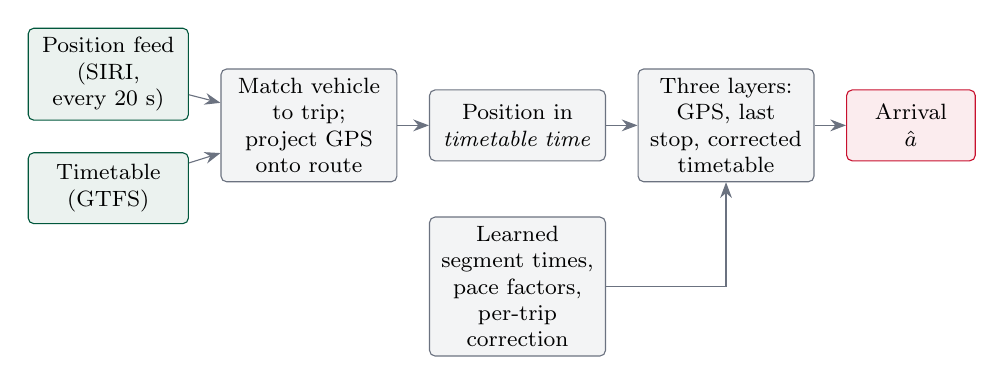
\begin{tikzpicture}[node distance=4mm and 4mm, every node/.style={font=\footnotesize},
  caja/.style={draw=gris, rounded corners=2pt, fill=gris!8, align=center, minimum height=9mm, text width=20mm},
  dato/.style={draw=ruta, rounded corners=2pt, fill=ruta!8, align=center, minimum height=9mm, text width=18mm},
  flecha/.style={-{Stealth[length=2mm]}, gris}]
\node[dato] (feed) {Position feed\\(SIRI, every 20 s)};
\node[dato, below=of feed] (gtfs) {Timetable\\(GTFS)};
\node[caja, right=of feed, yshift=-6.5mm] (match) {Match vehicle to trip; project GPS onto route};
\node[caja, right=of match] (tt) {Position in \emph{timetable time}};
\node[caja, right=of tt] (layers) {Three layers:\\GPS, last stop, corrected timetable};
\node[caja, below=of tt, yshift=-3mm] (learn) {Learned segment times, pace factors, per-trip correction};
\node[dato, right=of layers, text width=14mm, draw=gps, fill=gps!8] (eta) {Arrival\\$\hat a$};
\draw[flecha] (feed) -- (match);
\draw[flecha] (gtfs) -- (match);
\draw[flecha] (match) -- (tt);
\draw[flecha] (tt) -- (layers);
\draw[flecha] (learn) -| (layers);
\draw[flecha] (layers) -- (eta);
\end{tikzpicture}
\caption{Outline of the Bide+ method \parencite{garrido2026memoria,garrido2026metodo}. Only the operator's open data enter
it: the position feed and the timetable.}
\label{fig:method}
\end{figure}

The report \parencite{garrido2026memoria} gives every constant and the measurements behind it. The production engine is
not public; an open reference implementation in Python agrees with it on all 407 test vectors produced by that engine, and
it is the implementation used here. Against the published timetable, over 9.1 million predictions in 23 days, the method
was within $\pm2$~minutes in 92--96\% of cases with the bus less than three minutes away and in 67\% at 10 to 20 minutes,
against 23--25\% for the timetable \parencite{garrido2026metodo}.

% =====================================================================================================================
\section{Data}
\label{sec:data}

\subsection{What was captured}

A program running on GitHub Actions captured, during service hours:
\begin{itemize}
  \item \textbf{The live feed}, every 20 seconds: the public SIRI Vehicle Monitoring file of Bizkaibus, with the GPS
        position, the trip and the next stop of every vehicle in service. The file changes every 60 seconds.
  \item \textbf{The official waiting times}, about once a minute for each of 60 stops: the full response of the official
        web service, queried stop after stop (about one request per second in total), with the time $t$ at which each
        request was sent and the response latency (median 0.97~s).
\end{itemize}
The timetable is the Bizkaibus GTFS published on 25 September 2026 and valid until 24 November 2026, which covers the week;
the database built from it is published with the data.

\subsection{Stops}

The 60 stops, 28 of them \emph{priority} stops, were chosen before the capture. The 32 other stops are intermediate stops with many buses and lines. Each is reached at least 15 minutes after the
start of the trip (median over its scheduled trips), and its name in the official service matches the timetable. The 28 priority stops are stops that passengers asked about (in San Juan, Durango
and Elorrio) and the Bilbao stops where, in earlier captures, the actual passage deviated most from the published time.
Because this second criterion could favour a method that corrects the timetable, results are also given without the
priority stops. Each stop and the reason for its choice are listed in the repository.

\subsection{Days}

The week runs from Sunday 8 to Saturday 14 November 2026 (Table~\ref{tab:days}). Only queries sent between 06:00 and 23:00
are used. Wednesday 11 was a general strike with minimum service; it is analysed separately. Monday 9 lacks its morning (the
capture overran the time limit of its job), and Thursday 12 lacks official times after 17:12: the service stopped answering
over HTTP, and the capture has used HTTPS since, at the same request rate and without further failures. Saturday 14, whose
capture started at 09:41, is not part of this analysis. The feed has two gaps longer than two minutes, of 21 minutes on
Monday 9 (18:17--18:38) and of 203~s on Tuesday 10; no passage is reconstructed across them (Section~\ref{sec:passage}).

\begin{table}[t]
\centering
\caption{Days of the capture (Madrid time). Only queries sent between 06:00 and 23:00 are analysed.}
\label{tab:days}
\small
\begin{tabularx}{\linewidth}{llX}
\toprule
Date & Day & Coverage \\
\midrule
8 Nov 2026 & Sunday & From 06:46 \\
9 Nov 2026 & Monday & From 12:42 (morning lost: the capture overran its time limit); feed gap 18:17--18:38 \\
10 Nov 2026 & Tuesday & Complete; feed gap of 203~s; an early block before 06:00 is not used \\
11 Nov 2026 & Wednesday & Complete, \emph{analysed separately}: general strike, minimum services (about 30\%) \\
12 Nov 2026 & Thursday & Feed complete; official times until 17:12 (the service stopped answering over HTTP) \\
13 Nov 2026 & Friday & Complete (official times over HTTPS) \\
14 Nov 2026 & Saturday & From 09:41 (the scheduled start of the capture did not run) \\
\bottomrule
\end{tabularx}
\end{table}


% =====================================================================================================================
\section{Comparison design}
\label{sec:design}

\subsection{The three predictions}

For a query sent at time $t$ to stop $s$, and the bus matched to it (Section~\ref{sec:matching}):
\begin{itemize}
  \item \textbf{Timetable:} $\hat a_{\mathrm{tt}}$, the published time of the bus's trip at $s$.
  \item \textbf{Official:} $\hat a_{\mathrm{off}} = t + 60\,m$, where $m$ is the announced waiting time in minutes. Whether
        the service rounds or truncates $m$ is unknown; truncation is tested in the sensitivity analysis.
  \item \textbf{Bide+:} the prediction of the reference implementation in the last copy of the feed before $t$, at most
        60 seconds old (median 28~s, a small handicap for Bide+), with the learned tables of Saturday 7 November,
        calibrated only with data from before the week and not updated during it. It is rounded to whole minutes from
        $t$ as the app shows it, $\hat a_{\mathrm{B+}} = t + 60\max(0, [(\hat a - t)/60])$, halves away from zero.
\end{itemize}

\subsection{The actual passage}
\label{sec:passage}

\paragraph{From the feed} The actual passage $a$ of a bus at a stop is the midpoint between the last copy of the feed in
which the next stop of the bus is $s$ or an earlier one and the first copy in which it is a later one, without the bus
changing trip. The bus may be missing from the feed for up to five minutes in between, but the two bracketing copies of
the feed must be at most 90~s apart, so no passage is interpolated across a gap. Trips are identified by their full feed
reference (line, trip number and departure time), because Bizkaibus reuses trip numbers within a day. Since the feed
changes every 60 seconds, $a$ is known to within about $\pm30$~s.

\paragraph{From GPS} This definition uses the same feed field that Bide+ uses. An independent passage $a_{\mathrm{GPS}}$
is therefore computed from the positions alone: the moment of closest approach of the bus to the stop, interpolated between
the two positions that bracket the stop, if one of them is within 500~m. It is available for 99.7\% of the pairs. The two
agree closely: $a_{\mathrm{GPS}} - a$ has a median of $-4$~s, its 10th and 90th percentiles are $-36$ and $+34$~s, and
89\% of the differences are within one minute. The main analysis uses $a$; $a_{\mathrm{GPS}}$ is used as an alternative
ground truth.

\paragraph{Failed reconstructions} A pair is discarded if $a$ and $a_{\mathrm{GPS}}$ differ by more than five minutes, or
if reaching the stop by $a$ would require travelling at more than 30~m/s from the smaller of two distances at $t$: the
straight-line distance of the bus in the feed (a lower bound on the road distance) and the distance reported by the
official service, allowing 60~s for the feed's resolution. This removes 1.9\% of the
eligible pairs. One stop, Atxuri (3394), where all three sources were off by the same 17 to 30 minutes, which points to a
failure of the reconstruction rather than of the predictors, is excluded entirely. This exclusion was decided after
inspecting the errors; the sensitivity analysis that keeps it changes no conclusion (Table~\ref{tab:sensitivity}).

\subsection{Matching announcements to buses}
\label{sec:matching}

The official service does not identify the vehicle it announces. For a query at $t$ to stop $s$, its first announcement for
line $\ell$ (called $e_1$) is matched to the first bus of line $\ell$, among those tracked in the feed, that actually passes
$s$ after $t$, and its second announcement ($e_2$) to the second; passages up to 60 minutes after $t$ are considered. The
match is accepted only if the distance that the official service gives for the announced bus is consistent with the
straight-line distance of the matched bus from the stop in the feed: within 500~m, or between 0.6 and 2 times it. The
official distance appears to be measured along the road: for buses more than 1~km away, its ratio to the straight-line
distance has a median of 1.28 (10th and 90th percentiles 0.97 and 1.91). The check rejects a median of 6\% of the pairs
per stop (at most 37\%). A stricter version, within 300~m or between 0.9 and 1.6 times, is reported as a sensitivity
analysis. Lines listed twice in the same response would be left out; there were none. No stop is visited twice by the same trip,
but 12 of the 60 stops are the last stop of some routes; a bus ending its trip there has no reconstructed passage, so an
announcement for it would be matched to the next bus. Such a mismatch makes the official error negative, the opposite of
the bias observed (Section~\ref{sec:tails}), and most are rejected by the distance check.

When the matched bus is not in the feed at $t$, Bide+ can only give a fallback prediction and the bus's distance is
unknown, so the identity check cannot be applied. These pairs are excluded from the main analysis and included in a
sensitivity analysis.

\subsection{Metrics and inference}

The error of each prediction is $\hat a - a$: positive when the bus arrives \emph{earlier} than predicted. The main scoring
rule is the share of predictions within $\pm2$~minutes, chosen in advance as in the companion paper. It is a threshold
rule of the kind that suits a decision with a tolerance \parencite{gneiting2011point}. The median and mean absolute errors,
the shares within $\pm1$ and $\pm3$~minutes, the median signed error and the share of buses that arrive more than two
minutes early are also reported. The main analysis uses pairs with $0 \le a - t < 30$~min, by actual time to arrival;
results by the announced time $m$ use all announcements of up to 29 minutes whose bus passed within the next hour.
These rules (the 90-second gap rule, the identity check, the failed-reconstruction rule and the Atxuri exclusion) were
set after the data had been collected and inspected; each is varied in the sensitivity analysis.

Predictions of the same trip, and of the same stop, are not independent: one passage contributes a prediction every
minute. Confidence intervals for the difference in the share within $\pm2$~minutes are percentile intervals from 2,000
bootstrap resamples of whole trips and, separately, of whole stops \parencite{efron1993bootstrap}. The mean loss
differential $d = |e_{\mathrm{off}}| - |e_{\mathrm{B+}}|$ is tested with standard errors clustered by stop and by stop and
day, in the manner of \textcite{diebold1995comparing}. With five days, day-level variance cannot be estimated.

\paragraph{Passenger model} A passenger is assumed to reach the stop $k$ minutes before the predicted arrival
($k = 1, 2, 3$). If the bus has already passed, the passenger waits for the next bus of the same line. The model reports
the share of missed buses and the expected wait including that cost, for announcements of 3 to 29 minutes.

% =====================================================================================================================
\section{Results}
\label{sec:results}

\subsection{Pairs and coverage}

Of the official announcements of the next bus less than 30 minutes ahead on the five normal days (720,567), 74.0\% could
be paired with a bus whose actual passage was observed, and 54.8\% passed the identity check and entered the main
analysis. The main analysis has 484,026 pairs: 25,843 passages of 9,137 trips, made by 316 vehicles on 73 lines, at 59
stops, with between 199 and 281 different vehicles in each hour from 06:00 to 22:00. Table~\ref{tab:flow} in
\ref{app:extra} follows the pairs by day.

\subsection{Accuracy by time to arrival}

\begin{figure}[t]
\centering
\begin{tikzpicture}
\begin{axis}[
  name=arriba, width=0.95\textwidth, height=5.6cm,
  ylabel={Within $\pm2$ min (\%)},
  xmin=0, xmax=30, ymin=0, ymax=100, xtick={0,5,...,30}, xticklabels={},
  axis lines*=left, ymajorgrids, grid style={gris!20},
  tick label style={font=\footnotesize}, label style={font=\small},
  legend style={font=\footnotesize, draw=none, fill=none, at={(0.98,0.98)}, anchor=north east}]
\addplot[ruta, very thick] table[x=min, y=met] {figuras/minutos.dat};
\addlegendentry{Bide+}
\addplot[gps, very thick, dashed] table[x=min, y=ofi] {figuras/minutos.dat};
\addlegendentry{Official real time}
\addplot[gris, very thick, dotted] table[x=min, y=hor] {figuras/minutos.dat};
\addlegendentry{Published timetable}
\end{axis}
\begin{axis}[
  at={(arriba.below south west)}, anchor=north west, yshift=-2mm,
  width=0.95\textwidth, height=3.6cm,
  xlabel={Minutes to the actual passage}, ylabel={\shortstack{Bide+ $-$ official\\(points)}},
  xmin=0, xmax=30, ymin=-10, ymax=45, xtick={0,5,...,30},
  axis lines*=left, ymajorgrids, grid style={gris!20},
  tick label style={font=\footnotesize}, label style={font=\small}]
\addplot[name path=hi, draw=none] table[x=min, y=difhi] {figuras/minutos.dat};
\addplot[name path=lo, draw=none] table[x=min, y=diflo] {figuras/minutos.dat};
\addplot[ruta!30] fill between[of=hi and lo];
\draw[gris] (axis cs:0,0) -- (axis cs:30,0);
\end{axis}
\end{tikzpicture}
\caption{Top: share of predictions within two minutes of the actual passage, by minutes to that passage (one-minute bins).
Bottom: 95\% bootstrap interval (2,000 resamples of trips per bin) of the difference, Bide+ minus official, in percentage
points. Main analysis, 484,026 pairs.}
\label{fig:minutes}
\end{figure}

\begin{table}[t]
\centering
\caption{Errors of the three sources by time to the actual passage. \emph{Med.}: median absolute error (s). \emph{$\pm$2}:
share within two minutes (\%). \emph{Early}: share of buses arriving more than two minutes before the predicted time
(\%; error $\hat a - a > 120$~s).}
\label{tab:horizon}
\footnotesize
\setlength{\tabcolsep}{2.6pt}
\begin{tabular}{lrrrrrrrrrr}
\toprule
 & & \multicolumn{3}{c}{Timetable} & \multicolumn{3}{c}{Official real time} & \multicolumn{3}{c}{Bide+} \\
\cmidrule(lr){3-5}\cmidrule(lr){6-8}\cmidrule(lr){9-11}
Minutes & Pairs & Med. & $\pm$2 & Early & Med. & $\pm$2 & Early & Med. & $\pm$2 & Early \\
\midrule
\csname @@input\endcsname tablas/horizonte.tex
\bottomrule
\end{tabular}
\end{table}

The published timetable is within two minutes of the actual passage in 14--19\% of cases at every horizon, with a median
absolute error of six to eight minutes (Table~\ref{tab:horizon}, Figure~\ref{fig:minutes}). With the bus less than three
minutes away, the official real time and Bide+ are equally accurate: 92\% of their predictions are within two minutes
(difference $-0.6$ to $+0.2$ points, 95\% interval by trip). From three minutes on, Bide+ is more often within two minutes:
82\% against 59\% at 3--6 minutes, 75\% against 42\% at 6--10, 63\% against 31\% at 10--20 and 49\% against 23\% at 20--30
minutes. Over all horizons the shares are 16\% for the timetable, 41\% for the official real time and 67\% for Bide+, and
the ordering is the same within one and within three minutes (Table~\ref{tab:metrics} in \ref{app:extra}).

\subsection{Inference}

\begin{table}[t]
\centering
\caption{Inference. Columns 2--3: 95\% bootstrap intervals (2,000 resamples) of the difference Bide+ minus official in
the share within two minutes (percentage points), resampling trips or stops. Columns 4--6: mean loss differential
$d = |e_{\mathrm{off}}| - |e_{\mathrm{B+}}|$ (s; positive favours Bide+) and $z = d/\mathrm{SE}$ with standard errors
clustered by stop or by stop and day.}
\label{tab:inference}
\footnotesize
\begin{tabular}{lrrrrr}
\toprule
Minutes & By trip & By stop & $d$ (s) & $z$ (stop) & $z$ (stop-day) \\
\midrule
\csname @@input\endcsname tablas/inferencia.tex
\bottomrule
\end{tabular}
\end{table}

From three minutes on, the difference in the share within two minutes is positive with either clustering; the lowest
lower bound, by stop at 3--6 minutes, is 16 points (Table~\ref{tab:inference}). The mean absolute
error gives a more nuanced picture. Below six minutes the official real time has the smaller mean absolute error, because
Bide+ has more very large errors (Section~\ref{sec:tails}); between 6 and 10 minutes the two do not differ; from 10 minutes
on Bide+ has the smaller mean absolute error, by 76 to 141~s. Bide+ is therefore more often close to the actual passage
from three minutes on, while its mean error is smaller only from ten.

\subsection{Accuracy by announced waiting time}

A passenger sees the announced time, not the actual one. Table~\ref{tab:announced} bins all announcements of up to 29
minutes by the minutes announced. The ranking is the same: when the official service announced 6 to 9 minutes, its
announcement was within two minutes of the actual passage in 54\% of cases and Bide+ in 76\%; at 10 to 19 minutes, 37\% and
65\%; at 20 to 29 minutes, 23\% and 52\%. Over all these announcements the shares are 17\%, 44\% and 67\%.

\begin{table}[t]
\centering
\caption{Errors of the three sources by the waiting time announced by the official service (minutes, $m \le 29$; buses
passing within the next hour). Columns as in Table~\ref{tab:horizon}.}
\label{tab:announced}
\footnotesize
\setlength{\tabcolsep}{2.6pt}
\begin{tabular}{lrrrrrrrrrr}
\toprule
 & & \multicolumn{3}{c}{Timetable} & \multicolumn{3}{c}{Official real time} & \multicolumn{3}{c}{Bide+} \\
\cmidrule(lr){3-5}\cmidrule(lr){6-8}\cmidrule(lr){9-11}
Announced & Pairs & Med. & $\pm$2 & Early & Med. & $\pm$2 & Early & Med. & $\pm$2 & Early \\
\midrule
\csname @@input\endcsname tablas/anunciado.tex
\bottomrule
\end{tabular}
\end{table}

\subsection{Robustness to the ground truth}

With the GPS-based passage as ground truth, the shares within two minutes are 16\%, 42\% and 69\%, and below three minutes
Bide+ is slightly ahead (95\% against 94\%; Table~\ref{tab:gps} in \ref{app:extra}). Shifting the feed-based passage
(Figure~\ref{fig:shift} in \ref{app:extra}) shows that Bide+ fits best when the passage is taken 30~s earlier and the
official real time when it is taken as is. Bide+ stays ahead unless the true passage were more than two minutes later than
reconstructed, an offset that the agreement with the GPS-based passage rules out. The ranking is also unchanged in the
other 11 sensitivity analyses (Table~\ref{tab:sensitivity} in \ref{app:extra}): official minutes truncated rather than
rounded, Bide+ in seconds or truncated, a stricter identity check or none, with the fallback pairs, without Zabalburu, with
the excluded stop and failed passages, one random pair per passage, without the priority stops, and with live positions
only.

\subsection{Direction and size of the errors}
\label{sec:tails}

\begin{figure}[t]
\centering
\begin{tikzpicture}
\begin{axis}[
  name=cdf, width=0.5\textwidth, height=5.6cm,
  xlabel={Absolute error (min)}, ylabel={Predictions with smaller error (\%)},
  xmin=0, xmax=15, ymin=0, ymax=100, xtick={0,2,...,14},
  axis lines*=left, grid=major, grid style={gris!15},
  tick label style={font=\footnotesize}, label style={font=\small},
  legend style={font=\scriptsize, draw=none, fill=none, at={(0.98,0.03)}, anchor=south east}]
\addplot[ruta, very thick] table[x=min, y=met] {figuras/cdf.dat};
\addlegendentry{Bide+}
\addplot[gps, very thick, dashed] table[x=min, y=ofi] {figuras/cdf.dat};
\addlegendentry{Official}
\addplot[gris, very thick, dotted] table[x=min, y=hor] {figuras/cdf.dat};
\addlegendentry{Timetable}
\end{axis}
\begin{axis}[
  at={(cdf.east)}, anchor=west, xshift=14mm,
  width=0.5\textwidth, height=5.6cm,
  xlabel={Error $\hat a - a$ (min)}, ylabel={Predictions (\%)},
  xmin=-10, xmax=10, ymin=0, xtick={-10,-5,0,5,10},
  axis lines*=left, ymajorgrids, grid style={gris!20},
  tick label style={font=\footnotesize}, label style={font=\small}]
\addplot[const plot mark mid, ruta, very thick] table[x=min, y=met] {figuras/errores.dat};
\addplot[const plot mark mid, gps, very thick, dashed] table[x=min, y=ofi] {figuras/errores.dat};
\addplot[const plot mark mid, gris, very thick, dotted] table[x=min, y=hor] {figuras/errores.dat};
\end{axis}
\end{tikzpicture}
\caption{Errors with the bus 10 to 20 minutes away (legend in the left panel). Left: cumulative distribution of the
absolute error. Right: distribution of the signed error in 30-second bins; positive means the bus arrives earlier than
predicted. Beyond $+10$ minutes lie 33.8\% of timetable, 10.6\% of official and 1.4\% of Bide+ predictions; below $-10$
minutes, 4.8\%, 0.5\% and 0.5\%.}
\label{fig:errors}
\end{figure}

The timetable errs in one direction: buses run ahead of it (median signed error $+334$~s at 10--20 minutes), and 63\% of
them pass more than two minutes before the published time. The official real time keeps that direction with less than
half the size ($+132$~s): in about half of the cases at 10 to 30 minutes, the bus passes more than two minutes before the
announced time. Bide+ is nearly centred ($-32$~s at 10--20 minutes), and the bus is more than two minutes early in 12\% of
cases at those horizons (Figure~\ref{fig:errors}; Table~\ref{tab:horizon-extra} in \ref{app:extra}).

Bide+ has, however, more very large errors at short horizons: with the bus less than six minutes away, 1.7--1.8\% of its
predictions are more than ten minutes off, against 0.1--1.1\% for the official real time (Table~\ref{tab:tails} in
\ref{app:extra}). Of these 2,030 errors, 832 occur at one Bilbao stop (Zabalburu, 305), and two thirds come from its
fallback layers: the bus was in the feed, but the GPS layer abstained and Bide+ used the last reported stop or the
corrected timetable. Without that stop the shares within two minutes are unchanged (41\% and
67\%; Table~\ref{tab:sensitivity}).

\subsection{Consequences for a passenger}

\begin{table}[t]
\centering
\caption{Passenger model, announcements of 3 to 29 minutes: a passenger reaches the stop $k$ minutes before the predicted
arrival and, if the bus has gone, waits for the next one of the same line. \emph{Miss}: share of missed buses (\%).
\emph{Wait}: expected wait including misses (min).}
\label{tab:passenger}
\footnotesize
\begin{tabular}{lrrrrrr}
\toprule
 & \multicolumn{2}{c}{Timetable} & \multicolumn{2}{c}{Official} & \multicolumn{2}{c}{Bide+} \\
\cmidrule(lr){2-3}\cmidrule(lr){4-5}\cmidrule(lr){6-7}
$k$ & Miss & Wait & Miss & Wait & Miss & Wait \\
\midrule
\csname @@input\endcsname tablas/viajero.tex
\bottomrule
\end{tabular}
\end{table}

A passenger who arrives two minutes before the predicted time misses the bus in 58\% of cases when following the
timetable, 37\% with the official real time and 9\% with Bide+. Counting the wait for the next bus when the first is
missed, the expected wait is 19.9, 18.1 and 5.3 minutes (Table~\ref{tab:passenger}). The ranking holds for every margin.
The model is deliberately simple: it ignores that a passenger may see an updated prediction on the way to the stop.

\subsection{San Juan (Amorebieta)}

\begin{figure}[t]
\centering
\begin{tikzpicture}
\pgfplotsset{sj/.style={width=0.5\textwidth, height=4.6cm, axis lines*=left, ymajorgrids, grid style={gris!20},
  tick label style={font=\scriptsize}, label style={font=\scriptsize}, title style={font=\scriptsize}}}
\begin{axis}[sj, name=s1, x dir=reverse, xmin=0, xmax=30, ymin=0, ymax=45, xtick={30,20,10,0},
  title={Direction 1: stop 3388, line 3514, Mon 9}, ylabel={Predicted wait (min)},
  xlabel={Minutes before the actual passage}]
\addplot[gris, thin, domain=0:30] {x};
\addplot[ruta, thick, mark=*, mark size=0.9pt] table[x=antes, y=met] {figuras/sanjuan1.dat};
\addplot[gps, thick, dashed, mark=square*, mark size=0.9pt] table[x=antes, y=ofi] {figuras/sanjuan1.dat};
\addplot[gris, thick, dotted] table[x=antes, y=hor] {figuras/sanjuan1.dat};
\end{axis}
\begin{axis}[sj, name=s2, at={(s1.east)}, anchor=west, xshift=10mm, x dir=reverse, xmin=0, xmax=30, ymin=0, ymax=45,
  xtick={30,20,10,0}, title={Direction 2: stop 3391, line 3513, Thu 12}, xlabel={Minutes before the actual passage},
  legend style={font=\scriptsize, draw=none, fill=none, at={(-0.12,1.22)}, anchor=south, legend columns=4,
    /tikz/every even column/.append style={column sep=3mm}}]
\addplot[gris, thin, domain=0:30] {x};
\addlegendentry{Perfect}
\addplot[ruta, thick, mark=*, mark size=0.9pt] table[x=antes, y=met] {figuras/sanjuan2.dat};
\addlegendentry{Bide+}
\addplot[gps, thick, dashed, mark=square*, mark size=0.9pt] table[x=antes, y=ofi] {figuras/sanjuan2.dat};
\addlegendentry{Official}
\addplot[gris, thick, dotted] table[x=antes, y=hor] {figuras/sanjuan2.dat};
\addlegendentry{Timetable}
\end{axis}
\begin{axis}[sj, name=s3, at={(s1.below south west)}, anchor=north west, yshift=-12mm,
  ybar, bar width=6pt, ymin=0, ymax=100, ylabel={Within $\pm2$ min (\%)}, title={By line (bus 3 to 30 min away)},
  symbolic x coords={3513,3514,3515}, xtick=data, enlarge x limits=0.25]
\addplot[fill=ruta, draw=ruta] table[x=linea, y=met] {figuras/sanjuan-lineas.dat};
\addplot[fill=gps, draw=gps] table[x=linea, y=ofi] {figuras/sanjuan-lineas.dat};
\addplot[fill=gris!60, draw=gris] table[x=linea, y=hor] {figuras/sanjuan-lineas.dat};
\end{axis}
\begin{axis}[sj, at={(s3.east)}, anchor=west, xshift=10mm, xmin=0, xmax=30, ymin=0, ymax=100, xtick={0,5,...,30},
  title={By minutes to the actual passage}, xlabel={Minutes to the actual passage}]
\addplot[ruta, very thick, mark=*, mark size=1.2pt] table[x=min, y=met] {figuras/sanjuan-horizonte.dat};
\addplot[gps, very thick, dashed, mark=square*, mark size=1.2pt] table[x=min, y=ofi] {figuras/sanjuan-horizonte.dat};
\addplot[gris, very thick, dotted] table[x=min, y=hor] {figuras/sanjuan-horizonte.dat};
\end{axis}
\end{tikzpicture}
\caption{San Juan (Amorebieta), lines 3513 to 3515 in both directions. Top: predicted against actual waiting time for one
bus drawn at random in each direction (fixed seed) among the passages with queries from at least 25 minutes before; the
thin line is a perfect prediction. Bottom: share within two minutes by line (bars: Bide+, official, timetable) and by
minutes to the actual passage (points at the middle of the bins of Table~\ref{tab:horizon}). Main analysis.}
\label{fig:sanjuan}
\end{figure}

San Juan, in Amorebieta, is one of the stops that passengers asked about, served in both directions by lines 3513 to 3515
(Figure~\ref{fig:sanjuan}). Over 8,298 pairs with the bus 3 to 30 minutes away, the timetable was within two minutes in
17\% of cases, the official real time in 33\% and Bide+ in 67\%, close to the network-wide figures for the same horizons
(15\%, 34\% and 63\%). The official real time was much less accurate in one direction (20\% at stop 3388) than in the other
(47\% at 3391), while Bide+ was similar in both (65\% and 70\%). The two buses drawn at random illustrate the aggregate pattern:
the timetable is offset by a roughly constant amount, the official real time is closer but announces the bus later than it
comes, and Bide+ follows the actual waiting time most closely. Four buses drawn at random from the whole network are shown in
Figure~\ref{fig:examples} in \ref{app:extra}.

\subsection{Stops, time of day and days}

\begin{figure}[t]
\centering
\begin{tikzpicture}
\begin{axis}[
  width=0.58\textwidth, height=0.58\textwidth,
  xlabel={Official: within $\pm2$ min (\%)}, ylabel={Bide+: within $\pm2$ min (\%)},
  xmin=0, xmax=100, ymin=0, ymax=100,
  axis lines*=left, grid=major, grid style={gris!15},
  tick label style={font=\footnotesize}, label style={font=\small},
  legend style={font=\footnotesize, draw=none, fill=none, at={(0.98,0.02)}, anchor=south east}]
\addplot[gris, domain=0:100] {x};
\addlegendentry{Equal accuracy}
\addplot[only marks, mark=*, ruta, scatter, scatter src=explicit, scatter/use mapped color={draw=ruta, fill=ruta!60},
  visualization depends on={sqrt(\thisrow{n})/25 \as \rad},
  scatter/@pre marker code/.append style={/tikz/mark size=\rad}, restrict expr to domain={\thisrow{prioritaria}}{0:0}]
  table[x=ofi, y=met, meta=n] {figuras/paradas.dat};
\addlegendentry{Other stop}
\addplot[only marks, mark=*, gps, scatter, scatter src=explicit, scatter/use mapped color={draw=gps, fill=gps!60},
  visualization depends on={sqrt(\thisrow{n})/25 \as \rad},
  scatter/@pre marker code/.append style={/tikz/mark size=\rad}, restrict expr to domain={\thisrow{prioritaria}}{1:1}]
  table[x=ofi, y=met, meta=n] {figuras/paradas.dat};
\addlegendentry{Priority stop}
\end{axis}
\end{tikzpicture}
\caption{Each point is one stop (bus 3 to 30 minutes away; marker radius proportional to the square root of the number of
pairs, on the same scale for both groups). Bide+ is more often within two minutes at 57 of the 59 stops, and at 56 the
95\% interval of the difference (2,000 resamples of trips) excludes zero.}
\label{fig:stops}
\end{figure}

The ranking is not confined to a few stops, hours or days. Bide+ is more often within two minutes than the official real
time at 57 of the 59 stops (Figure~\ref{fig:stops}). Of the other two, at Zabalburu (305) the two tie (35\%), and at Labakua
(2856) the timetable is the most accurate source (72\%, against 65\% official and 59\% Bide+). The ranking timetable,
official, Bide+ holds at every hour from 06:00 to 22:00 and on each of the five normal days
(Figure~\ref{fig:hours-days} in \ref{app:extra}), at the priority stops and at the others, on weekdays and on Sunday, and
for the second announced bus (Table~\ref{tab:groups}).

\subsection{Ablation: what makes Bide+ more accurate}

\begin{table}[t]
\centering
\caption{Ablation: share within two minutes (\%) on the same pairs, with Bide+ with all its learned tables, without any
of them, and without each one in turn.}
\label{tab:ablation}
\footnotesize
\setlength{\tabcolsep}{3pt}
\begin{tabular}{lrrrrrrr}
\toprule
 & & & \multicolumn{4}{c}{Bide+ without} & \\
\cmidrule(lr){4-7}
Minutes & Pairs & Official & all tables & segment times & pace factors & trip correction & Bide+ \\
\midrule
\csname @@input\endcsname tablas/ablacion.tex
\bottomrule
\end{tabular}
\end{table}

Table~\ref{tab:ablation} recomputes Bide+ on the same pairs without its learned tables. Without any of them, the arrival is
built from timetable differences only, and Bide+ is within two minutes in 33\% of cases, below the official real time
(41\%). Removing the learned segment times alone lowers it from 67\% to 38\%. Removing the per-trip correction costs one
point. Removing the pace factors changes nothing, because they act only where a segment has no learned time. On these pairs
and by this metric, the learned segment travel times are what puts Bide+ ahead of the operator; locating the bus in
timetable time is not enough on its own.

\subsection{The strike day}

On Wednesday 11, with minimum service, the ranking was the same as on normal days (Table~\ref{tab:days-results} in
\ref{app:extra}). Bide+ was more often early than on normal days (21\% against 8--17\%), which is consistent with buses
running faster than in the normal traffic its tables were learned from; this was not tested directly.

% =====================================================================================================================
\section{Discussion}
\label{sec:discussion}

\subsection{What the comparison shows}

On the buses compared, the published timetable is a poor guide to when the bus will come, the operator's real time removes
part of its error, and Bide+, built only on the operator's open data, is within two minutes of the actual passage more
often than the operator's real time from three minutes before arrival onwards. The gap is largest, about 32 percentage
points, with the bus 6 to 20 minutes away, the range in which a passenger decides when to leave for the stop. Below three
minutes the two are equally often within two minutes, and below six minutes Bide+ has a small share of very large errors
that the operator does not have, about two fifths of them at one stop.

\subsection{Possible explanations}

The ablation identifies the learned segment travel times as the component that puts Bide+ ahead; without them it falls
below the official real time. This is consistent with the timetable on this network running behind the buses, and with the
official real time keeping part of that bias (Figure~\ref{fig:errors}). How the official service computes its waiting
times is not published, so this paper cannot say why its errors take the form they do.

\subsection{Implications}

Operators that publish vehicle positions make possible independent predictions that, on this network and week, and for
the announcements that could be matched and confirmed (55\%), were more often within two minutes than their own. The most
direct implication is for evaluation: operators that also publish their predictions, for example as GTFS-Realtime trip
updates \parencite{gtfsrt} or SIRI estimated timetables, would allow their accuracy to be audited independently and
continuously, as done here by recording a web service. The timetable itself could also be improved: with most buses passing more than two minutes before the published time at
these stops, revising the intermediate times, or holding buses at timing points, would help both printed timetables and
any real-time system anchored to them. Journey planners that show the operator's figures unchanged inherit
their accuracy; none was measured here.

\subsection{Limitations}

\begin{itemize}
  \item \textbf{Coverage.} 55\% of the official announcements of the next bus less than 30 minutes ahead entered the main
        analysis (74\% could be paired at all). Pairs where Bide+ had no live position are excluded by construction from
        the main analysis; including them, without the identity check, gives 39\% and 65\% (Table~\ref{tab:sensitivity}).
  \item \textbf{Ground truth.} The main ground truth comes from the feed field that Bide+ also uses, and its learned
        segment times were fitted on passages defined in the same way, so Bide+ is calibrated to this definition and is
        more sensitive than the official real time to shifting it (Figure~\ref{fig:shift}). The GPS-based passage shares
        the feed's vehicle-to-trip assignment and clock. The GPS-based passage, which does
        not use that field, agrees with it to within a minute in 89\% of cases and gives the same ranking. Field
        observation was not possible.
  \item \textbf{Matching.} The official service does not identify the vehicle it announces. The distance check compares
        a road distance with a straight-line one; stricter or no checks do not change the ranking, but some mismatches may
        remain, and they would count against the official source.
  \item \textbf{Selection of stops.} The stops were chosen by the author; 28 of them partly because the timetable deviates
        most there. Results without them are the same (41\% and 67\%), but the stops are not a random sample of the
        network.
  \item \textbf{One week, one network.} Five normal days in November, one of them a Sunday. Day-level variance cannot be
        estimated, and other seasons, networks or operators may differ.
  \item \textbf{Replay, not the app; source of the official times.} Bide+ was recomputed with its reference implementation
        and frozen tables; the app was not measured. That the web service returns what the official app and the displays
        show was not verified independently.
  \item \textbf{Analytical choices.} The scoring rule, horizons and matching follow the companion paper, and the stops were
        fixed before the capture, but the study was not preregistered, and the rules for reconstructing passages and
        confirming matches were set after the data had been inspected. A confirmatory replication on another week, ideally
        by a third party, would strengthen the conclusions.
\end{itemize}

% =====================================================================================================================
\section{Conclusions}
\label{sec:conclusions}

For one week, at 59 stops of the Bizkaibus network, the official real-time waiting times were recorded minute by minute and
compared, bus by bus, with the published timetable and with the arrivals predicted by the Bide+ method from the operator's
open position feed and timetable. Over all horizons up to 30 minutes, the timetable was within two minutes of the actual
passage in 16\% of the paired cases, the official real time in 41\% and Bide+ in 67\%, with the same ranking against an
independent GPS-based ground truth. Below three minutes the two real-time sources were equally often within two minutes;
from three minutes on Bide+ was more often within two minutes at almost every stop, hour and day, although its mean error
was smaller only from ten minutes. An ablation attributes its advantage to its learned segment travel times. These results
apply to the 55\% of announcements that could be matched and confirmed, and they call for a replication on other periods
and networks.


% =====================================================================================================================
\appendix
\section{Supporting tables and figures}
\setcounter{table}{0}\setcounter{figure}{0}
\label{app:extra}

\begin{table}[h]
\centering
\caption{From official announcements to the pairs analysed, by day (first and second bus, queries 06:00--23:00).
\emph{Paired}: announcements matched to a bus whose passage was observed within 60 minutes. \emph{Beyond 30} and
\emph{Within 30}: that passage more or less than 30 minutes after the query. \emph{Fallback}: the bus was not in the feed
at $t$ (Bide+ gives its fallback prediction). \emph{Excl.}: excluded stop or failed reconstruction. \emph{Not conf.}:
distance check failed. \emph{Main}: pairs in the main analysis. *~General strike, not part of the main results.}
\label{tab:flow}
\scriptsize
\setlength{\tabcolsep}{3pt}
\begin{tabular}{lrrrrrrrr}
\toprule
Day & Queries & Paired & Beyond 30 & Within 30 & Fallback & Excl. & Not conf. & Main \\
\midrule
\csname @@input\endcsname tablas/flujo.tex
\bottomrule
\end{tabular}
\end{table}

\begin{table}[h]
\centering
\caption{Coverage of the official announcements of the first bus with an announced wait under 30 minutes (six normal
days, 06:00--23:00), by minutes announced: share paired with a bus whose passage was observed within 30 minutes, and share
in the main analysis (\%).}
\label{tab:coverage}
\footnotesize
\begin{tabular}{lrrr}
\toprule
Announced & Announcements & Paired & Main \\
\midrule
\csname @@input\endcsname tablas/cobertura.tex 
\bottomrule
\end{tabular}
\end{table}

\begin{table}[h]
\centering
\caption{Share within two minutes (\%) in the main analysis and in the paired announcements excluded from it (all
horizons up to 30 minutes, six normal days, excluded stop and failed reconstructions removed). For pairs whose bus was not
in the feed, Bide+ gives its fallback prediction.}
\label{tab:excluded}
\footnotesize
\begin{tabular}{lrrrr}
\toprule
Pairs & Number & Timetable & Official & Bide+ \\
\midrule
\csname @@input\endcsname tablas/excluidos.tex 
\bottomrule
\end{tabular}
\end{table}

\begin{table}[h]
\centering
\caption{Share within two minutes (\%) by decile of the ratio between the official distance and the straight-line distance
of the matched bus (main analysis, bus more than 500~m away). Bide+ is ahead in every decile, so the result does not
depend on the pairs whose identity is least certain.}
\label{tab:ratio}
\footnotesize
\begin{tabular}{lrrrr}
\toprule
Decile & Ratio & Pairs & Official & Bide+ \\
\midrule
\csname @@input\endcsname tablas/razon.tex 
\bottomrule
\end{tabular}
\end{table}

\begin{table}[h]
\centering
\caption{Further metrics, all horizons up to 30 minutes (main analysis).}
\label{tab:metrics}
\footnotesize
\begin{tabular}{lrrr}
\toprule
Metric & Timetable & Official & Bide+ \\
\midrule
\csname @@input\endcsname tablas/metricas.tex
\bottomrule
\end{tabular}
\end{table}

\begin{table}[h]
\centering
\caption{Share within one minute (\%) and median signed error (s) by time to the actual passage. A positive signed error
means that the bus arrives earlier than predicted.}
\label{tab:horizon-extra}
\footnotesize
\begin{tabular}{lrrrrrr}
\toprule
 & \multicolumn{2}{c}{Timetable} & \multicolumn{2}{c}{Official} & \multicolumn{2}{c}{Bide+} \\
\cmidrule(lr){2-3}\cmidrule(lr){4-5}\cmidrule(lr){6-7}
Minutes & $\pm$1 & Signed & $\pm$1 & Signed & $\pm$1 & Signed \\
\midrule
\csname @@input\endcsname tablas/horizonte_extra.tex
\bottomrule
\end{tabular}
\end{table}

\begin{table}[h]
\centering
\caption{Mean absolute error (s) and share of predictions more than ten minutes off (\%), by time to the actual passage.}
\label{tab:tails}
\footnotesize
\begin{tabular}{lrrrrrr}
\toprule
 & \multicolumn{2}{c}{Timetable} & \multicolumn{2}{c}{Official} & \multicolumn{2}{c}{Bide+} \\
\cmidrule(lr){2-3}\cmidrule(lr){4-5}\cmidrule(lr){6-7}
Minutes & MAE & $>$10 min & MAE & $>$10 min & MAE & $>$10 min \\
\midrule
\csname @@input\endcsname tablas/colas.tex
\bottomrule
\end{tabular}
\end{table}

\begin{table}[h]
\centering
\caption{With the GPS-based passage as ground truth: share within two minutes (\%) by time to that passage, and 95\%
bootstrap interval (2,000 resamples of trips) of the difference Bide+ minus official (percentage points).}
\label{tab:gps}
\footnotesize
\begin{tabular}{lrrrrr}
\toprule
Minutes & Pairs & Timetable & Official & Bide+ & Difference \\
\midrule
\csname @@input\endcsname tablas/gps.tex
\bottomrule
\end{tabular}
\end{table}

\begin{figure}[h]
\centering
\begin{tikzpicture}
\begin{axis}[
  width=0.62\textwidth, height=5.4cm,
  xlabel={Shift applied to the actual passage (s)}, ylabel={Within $\pm2$ min (\%)},
  xmin=-180, xmax=180, ymin=0, ymax=100, xtick={-180,-120,...,180},
  axis lines*=left, ymajorgrids, grid style={gris!20},
  tick label style={font=\footnotesize}, label style={font=\small},
  legend style={font=\scriptsize, draw=none, fill=none, at={(0.02,0.98)}, anchor=north west}]
\addplot[ruta, very thick, mark=*, mark size=1.2pt] table[x=s, y=met] {figuras/desplazamiento.dat};
\addlegendentry{Bide+}
\addplot[gps, very thick, dashed, mark=square*, mark size=1.2pt] table[x=s, y=ofi] {figuras/desplazamiento.dat};
\addlegendentry{Official}
\addplot[gris, very thick, dotted] table[x=s, y=hor] {figuras/desplazamiento.dat};
\addlegendentry{Timetable}
\draw[gris, dashed] (axis cs:-36,0) -- (axis cs:-36,100);
\draw[gris, dashed] (axis cs:34,0) -- (axis cs:34,100);
\end{axis}
\end{tikzpicture}
\caption{Share within two minutes, all horizons, when the feed-based actual passage is shifted by the amount shown
(positive: later). The dashed lines mark the 10th and 90th percentiles of the difference between the GPS-based and the
feed-based passage.}
\label{fig:shift}
\end{figure}

\begin{table}[h]
\centering
\caption{Sensitivity analyses: share within two minutes (\%) over all horizons and with the bus 10 to 20 minutes away.}
\label{tab:sensitivity}
\scriptsize
\setlength{\tabcolsep}{2.5pt}
\begin{tabular}{lrrrrrr}
\toprule
 & & \multicolumn{3}{c}{All horizons} & \multicolumn{2}{c}{10--20 min} \\
\cmidrule(lr){3-5}\cmidrule(lr){6-7}
Variant & Pairs & Timet. & Official & Bide+ & Official & Bide+ \\
\midrule
\csname @@input\endcsname tablas/sensibilidad.tex
\bottomrule
\end{tabular}
\end{table}

\begin{table}[h]
\centering
\caption{Errors by group, all horizons up to 30 minutes. Columns as in Table~\ref{tab:horizon}.}
\label{tab:groups}
\footnotesize
\setlength{\tabcolsep}{2.6pt}
\begin{tabular}{lrrrrrrrrrr}
\toprule
 & & \multicolumn{3}{c}{Timetable} & \multicolumn{3}{c}{Official real time} & \multicolumn{3}{c}{Bide+} \\
\cmidrule(lr){3-5}\cmidrule(lr){6-8}\cmidrule(lr){9-11}
Group & Pairs & Med. & $\pm$2 & Early & Med. & $\pm$2 & Early & Med. & $\pm$2 & Early \\
\midrule
\csname @@input\endcsname tablas/grupos.tex
\bottomrule
\end{tabular}
\end{table}

\begin{table}[h]
\centering
\caption{Errors by day, all horizons up to 30 minutes. Columns as in Table~\ref{tab:horizon}. *~General strike, shown for
reference and not part of the main results.}
\label{tab:days-results}
\footnotesize
\setlength{\tabcolsep}{2.6pt}
\begin{tabular}{lrrrrrrrrrr}
\toprule
 & & \multicolumn{3}{c}{Timetable} & \multicolumn{3}{c}{Official real time} & \multicolumn{3}{c}{Bide+} \\
\cmidrule(lr){3-5}\cmidrule(lr){6-8}\cmidrule(lr){9-11}
Day & Pairs & Med. & $\pm$2 & Early & Med. & $\pm$2 & Early & Med. & $\pm$2 & Early \\
\midrule
\csname @@input\endcsname tablas/dias.tex
\bottomrule
\end{tabular}
\end{table}

\begin{figure}[h]
\centering
\begin{tikzpicture}
\pgfplotsset{ejemplo/.style={width=0.5\textwidth, height=4.4cm, x dir=reverse, xmin=0, xmax=30, ymin=0, ymax=45,
  xtick={30,20,10,0}, axis lines*=left, ymajorgrids, grid style={gris!20}, tick label style={font=\scriptsize},
  label style={font=\scriptsize}, title style={font=\scriptsize}}}
\begin{axis}[ejemplo, name=e1, title={Line 3917, stop 2576, Sun 8}, ylabel={Predicted wait (min)}]
\addplot[gris, thin, domain=0:30] {x};
\addplot[ruta, thick, mark=*, mark size=0.9pt] table[x=antes, y=met] {figuras/ejemplo1.dat};
\addplot[gps, thick, dashed, mark=square*, mark size=0.9pt] table[x=antes, y=ofi] {figuras/ejemplo1.dat};
\addplot[gris, thick, dotted] table[x=antes, y=hor] {figuras/ejemplo1.dat};
\end{axis}
\begin{axis}[ejemplo, name=e2, at={(e1.east)}, anchor=west, xshift=8mm, title={Line 3527, stop 3437, Tue 10}]
\addplot[gris, thin, domain=0:30] {x};
\addplot[ruta, thick, mark=*, mark size=0.9pt] table[x=antes, y=met] {figuras/ejemplo2.dat};
\addplot[gps, thick, dashed, mark=square*, mark size=0.9pt] table[x=antes, y=ofi] {figuras/ejemplo2.dat};
\addplot[gris, thick, dotted] table[x=antes, y=hor] {figuras/ejemplo2.dat};
\end{axis}
\begin{axis}[ejemplo, name=e3, at={(e1.below south west)}, anchor=north west, yshift=-6mm,
  title={Line 3641, stop 270, Thu 12}, ylabel={Predicted wait (min)}, xlabel={Minutes before the actual passage}]
\addplot[gris, thin, domain=0:30] {x};
\addplot[ruta, thick, mark=*, mark size=0.9pt] table[x=antes, y=met] {figuras/ejemplo3.dat};
\addplot[gps, thick, dashed, mark=square*, mark size=0.9pt] table[x=antes, y=ofi] {figuras/ejemplo3.dat};
\addplot[gris, thick, dotted] table[x=antes, y=hor] {figuras/ejemplo3.dat};
\end{axis}
\begin{axis}[ejemplo, at={(e3.east)}, anchor=west, xshift=8mm, title={Line 3911, stop 264, Thu 12},
  xlabel={Minutes before the actual passage},
  legend style={font=\scriptsize, draw=none, fill=white, at={(0.02,0.98)}, anchor=north west}]
\addplot[gris, thin, domain=0:30] {x};
\addlegendentry{Perfect}
\addplot[ruta, thick, mark=*, mark size=0.9pt] table[x=antes, y=met] {figuras/ejemplo4.dat};
\addlegendentry{Bide+}
\addplot[gps, thick, dashed, mark=square*, mark size=0.9pt] table[x=antes, y=ofi] {figuras/ejemplo4.dat};
\addlegendentry{Official}
\addplot[gris, thick, dotted] table[x=antes, y=hor] {figuras/ejemplo4.dat};
\addlegendentry{Timetable}
\end{axis}
\end{tikzpicture}
\caption{Predicted against actual waiting time for four buses drawn at random from the whole network (fixed seed), among
the passages with queries from at least 25 minutes before. The thin line is a perfect prediction.}
\label{fig:examples}
\end{figure}

\begin{figure}[h]
\centering
\begin{tikzpicture}
\begin{axis}[
  name=horas, width=0.54\textwidth, height=5.4cm,
  xlabel={Hour of the query}, ylabel={Within $\pm2$ min (\%)},
  xmin=5.5, xmax=22.5, ymin=0, ymax=100, xtick={6,8,...,22},
  axis lines*=left, ymajorgrids, grid style={gris!20},
  tick label style={font=\footnotesize}, label style={font=\small},
  legend style={font=\scriptsize, draw=none, fill=none, at={(0.5,1.02)}, anchor=south, legend columns=3}]
\addplot[ruta, very thick, mark=*, mark size=1.2pt] table[x=hora, y=met] {figuras/horas.dat};
\addlegendentry{Bide+}
\addplot[gps, very thick, dashed, mark=square*, mark size=1.2pt] table[x=hora, y=ofi] {figuras/horas.dat};
\addlegendentry{Official}
\addplot[gris, very thick, dotted] table[x=hora, y=hor] {figuras/horas.dat};
\addlegendentry{Timetable}
\end{axis}
\begin{axis}[
  at={(horas.east)}, anchor=west, xshift=14mm,
  width=0.48\textwidth, height=5.4cm, ylabel={Within $\pm2$ min (\%)},
  ybar, bar width=3.5pt, ymin=0, ymax=100,
  symbolic x coords={{Sun 8},{Mon 9},{Tue 10},{Wed 11*},{Thu 12},{Fri 13},{Sat 14}},
  xtick=data, x tick label style={rotate=45, anchor=east, font=\scriptsize},
  axis lines*=left, ymajorgrids, grid style={gris!20},
  tick label style={font=\footnotesize}, label style={font=\small},
  legend style={font=\scriptsize, draw=none, fill=none, at={(0.5,1.02)}, anchor=south, legend columns=3}]
\addplot[fill=ruta, draw=ruta] table[x=dia, y=met] {figuras/dias.dat};
\addlegendentry{Bide+}
\addplot[fill=gps, draw=gps] table[x=dia, y=ofi] {figuras/dias.dat};
\addlegendentry{Official}
\addplot[fill=gris!60, draw=gris] table[x=dia, y=hor] {figuras/dias.dat};
\addlegendentry{Timetable}
\end{axis}
\end{tikzpicture}
\caption{Share within two minutes with the bus 3 to 30 minutes away. Left: by hour of the query (six normal days,
13,000 to 42,000 pairs per hour). Right: by day (*~general strike, not part of the main results).}
\label{fig:hours-days}
\end{figure}


\backmatter

% Generado por bib-a-bibtex.py a partir de declaraciones.tex: no editar a mano.
\section*{Declarations}
% =====================================================================================================================
\bmhead{Competing interests}

The author designed the Bide+ method and develops the independent Bide+ passenger information app that uses it, and
therefore has an interest in its results. The app is free to use; it accepts voluntary donations, which are used to pay
for the server that runs it, and the author receives no other income from it. To limit the effect of this interest on the evaluation, the method was frozen
before the test week, its predictions were recomputed with the public reference implementation, the analysis rules are
stated in Section~\ref{sec:design}, and all data and code are published so that the comparison can be repeated
independently. The author has no relationship with Bizkaibus, the Diputación Foral de Bizkaia or the operators of the
service.

\bmhead{Funding}

This research did not receive any specific grant from funding agencies in the public, commercial or not-for-profit
sectors.

\bmhead{Author contributions}

\textbf{Yeray Garrido}: Conceptualization, Methodology, Software, Data curation, Formal analysis, Investigation,
Visualization, Writing -- original draft, Writing -- review \& editing.

\bmhead{Ethics approval and consent}

Not applicable: the study involves no human participants and no personal data.

\bmhead{Data and code availability}

The capture program, the list of stops with the reason for each, the days and stops used and excluded, the comparison,
the tables and the figure data are in the folder \texttt{articulo-comparacion} of the repository
\url{https://github.com/Garridoparrayeray/bide-eta} (code under the MIT licence, texts and derived data under CC BY 4.0; see below for the raw official responses).
The timetable database used is in the repository (\texttt{datos/horario}). An archived copy of the code, the derived data and this
preprint is deposited on Zenodo (\doidatos). The raw captures (feed copies, official responses and the timetable of
each day) are not part of that record: they are assets of the release \texttt{comparacion-2026-11} of the GitHub
repository, under the terms given below. The position feed and the timetable are open data published by the Diputación Foral de Bizkaia and listed in
the Spanish National Access Point \parencite{nap}.

\bmhead{Data collection and terms of use}

The official waiting times were obtained from the public web service used by the official Bizkaibus app, which requires
no authentication. The capture queried it sequentially, about one request per second in total, with a user agent that
identifies the project, and only during service hours. No permission was sought from the operator. The capture first used the plain-HTTP address of the service; on 12
November at 17:12 that address stopped answering (requests timed out), and from 13 November the capture used the HTTPS
address of the same service. Over the week, 0.5\% of the requests failed (most of them on 12 November after 17:12), all by timeout or a closed
connection; no
error status, rate-limit or blocking response was received. The host serves no \texttt{robots.txt}, and no terms of use
for the web service or for redistributing its responses were found. The data contain no
personal information: only stop, line and vehicle identifiers. The raw official responses are not covered by the CC BY licence of the derived data: they are redistributed only for
research, with attribution, and will be removed if their publisher asks.


\bibliography{referencias-bibtex}

\end{document}
